\documentclass[a4paper,10pt]{article}
\usepackage[utf8]{inputenc}
\usepackage[colorinlistoftodos,prependcaption,textsize=tiny]{todonotes}

\usepackage{minted}

\usepackage{blkarray}
\usepackage{amsmath}

\usepackage{hyperref}

%opening
\title{SSR-viz - a toolbox to detect and visualize protein
subfamily specific residues}
\author{Paul Zierep}

\begin{document}

\maketitle

\begin{abstract}


\end{abstract}

Homologous proteins can be classified into protein families. The members of a family share a similar structure and sequence. Despite their inherent
similarity, individual members of the same family can adopt very specific functions, leading to a further division into subfamilies. These functional
differences can often be assigned to specific residues. This information can be used for various applications, such as function-based subfamily
classification, rational site-directed mutagenesis and general elucidation of mechanisms of action. Here we introduce a novel user-friendly open-source
software which allows for the identification and visualization of these residues.

\pagebreak
\tableofcontents
\pagebreak

\section{What is SSR-viz ?}

SSR-viz helps to detect residues which distinguish protein subfamilies from each other.
Therefore, SSR-viz needs a Multiple Sequence Alignment (MSA) of a protein family and a CSV file which defines the 
subfamilies in the alignment.
For each position in the alignment a score is computed which aims to highlight positions which are conserved in a 
subfamily but differ significantly opposed to another subfamily. 

\section{Installation}

\subsection{Standalone executables}

We implemented standalone 
executables for Windows (tested on windows 10) and Linux (tested on Ubunt 16.04).
These a much bigger then the pure python module, but ship everything needed out of
the Box. \\

\url{https://github.com/PhaBiFreiburg/SSR-viz/tree/master/standalone/}

\begin{itemize}
\item{Windows: exe.win-amd64-3.5.zip}
\item{Linux: exe.linux-x86\_64-3.5.tar.gz}
\end{itemize}


\subsection{Using Pip}

SSR-viz in implemented as a standalone GUI framework. It is entirely 
written in Python 3. The program was successfully installed on
Ubuntu 14.04/16.04/18.04 and Windows 10/8. It can be installed via PIP - the official python repository. 
To install SSR-viz open a terminal an type: 

\begin{minted}{bash}
pip3 install ssrviz
\end{minted}

Some packages, especially \textbf{wxPython} 
which are normally automatically installed
by PIP can make problems, as they are using system dependencies, which can 
lead to errors when missing. 
Good advice to install wxPython can be 
found at: \url{https://wxpython.org/pages/downloads/index.html}.
They also supply custom builds which work on Ubuntu 16.04 and various other
Linux systems.

Nevertheless wxPython needs some system dependencies on Linux:
They can be easily installed for Ubuntu 16.04:

\begin{minted}{bash}
sudo apt-get install libwebkitgtk-dev libgtk2.0-dev libsdl1.2-dev \
freeglut3 freeglut3-dev libnotify-dev libgstreamerd-3-dev \
libgl1-mesa-glx libglu1-mesa libgl1-mesa-dev libglu1-mesa-dev \
libgconf2-dev libsdl1.2-dev zlib1g-dev libjpeg62-dev
\end{minted}

In some cases the \textbf{matplotlib} might also need some Help with \textbf{tkinter}.

\begin{minted}{bash}
sudo apt-get install python3-tk
\end{minted}

Installation via Pip for Windows should work without additional installations.

\subsection{Clone from GitHub}

SSR-viz can also be cloned from GitHub \url{https://github.com/PhaBiFreiburg/SSR-viz}.
But then the dependencies need to be installed manually, 
see: \\
SSR-viz/documenation/requirements.txt

\subsection{Mafft}

The only external tool needed is mafft, an excellent alignment tool which is 
required to map protein structure indices to the alignment. SSR-viz runs
without mafft, but for the \textbf{Add\_pdb} tool the mafft executable needs 
to be assigned (see section~\ref{add_p}).
Dont't worry mafft is easy to install on all systems:

\url{https://mafft.cbrc.jp/alignment/software/}

\section{Getting started}

In Section~\ref{example} a detailed use case is demonstrated, which shows
the usage of each tool as well as the input and output formats.
The use case can be reproduced with the provided files in
 \url{https://github.com/PhaBiFreiburg/SSR-viz/use_case} \todo{url ?}.

The SSR-viz algorithm is based on a multiple sequence alignment (MSA) file in 
FASTA format, which can be generated with various tools, such as Clustalo 
and Mafft or with a Webserver such as 
\href{https://zeus.cmm.msu.ru/#scenario=2}{Mustguseal} or 
\href{http://prodata.swmed.edu/promals3d/promals3d.php}{PROMALS3D}.

The topic of sequence alignment is beyond the scope of this manual.  
Nevertheless one should keep in mind that 
the quality of the alignment is crucial for the detection algorithm.
(Is is difficult to interpret the importance of a position, which has
more gaps then amino acids.)

Please provide the alignment in FASTA format, most tools allow this format as
an output option.

The first step is the classification of the sequences into subfamilies.
This is undoubtedly the most difficult part, as it often requires 
to identify the specific functionality based on scientific literature
or even undertake experimental validation. Dedicated databases such as 
\href{https://www.uniprot.org/}{UniProt} and \href{http://www.pantherdb.org/downloads/index.jsp}{PANTHER} 
can help to identify 
detailed protein functionality. 

Even though there are various tools available that can cluster protein sequences, 
these clustering methods always apply some kind of similarity scoring,
which leads in most cases to a clustering based on evolutionary relationship 
rather then functional similarity. 
This is demonstrated on an example in section~\ref{example}.

Ones you collected the class information of your sequences you can add
them to your alignment. The \textbf{CSV\_Builder} tool allows to creates 
a comma separated value (CSV) file which can be used to add the subfamily 
class label to the sequences
(see section~\ref{csv_b}).

An alignment and the CSV file is everything needed to 
detect subfamily specific residues in the sequences. 
The \textbf{SSR\_plot} tool handles the actual execution of the detection
algorithm, the output can be a mathplotlib \todo{cite} style plot (see section~\ref{ssr_p})
as pdf, a Javlview annotation file (which can show the results together with the 
alignment) as well as a 'stats.csv' file which summarizes the SSRs.

In most cases it is desired to observe the SSRs in a structural context.
Therefore, we also developed a tool \textbf{Add\_pdb} which allows
to map the indices of a protein structure file (*.pdb) to the indices of the 
alignment in the 'stats.csv' file (see section~\ref{add_p}).

An overview chart which explains the setup of the three tools is shown in
the figure~\ref{fig:flow_chart}.

\begin{figure}
  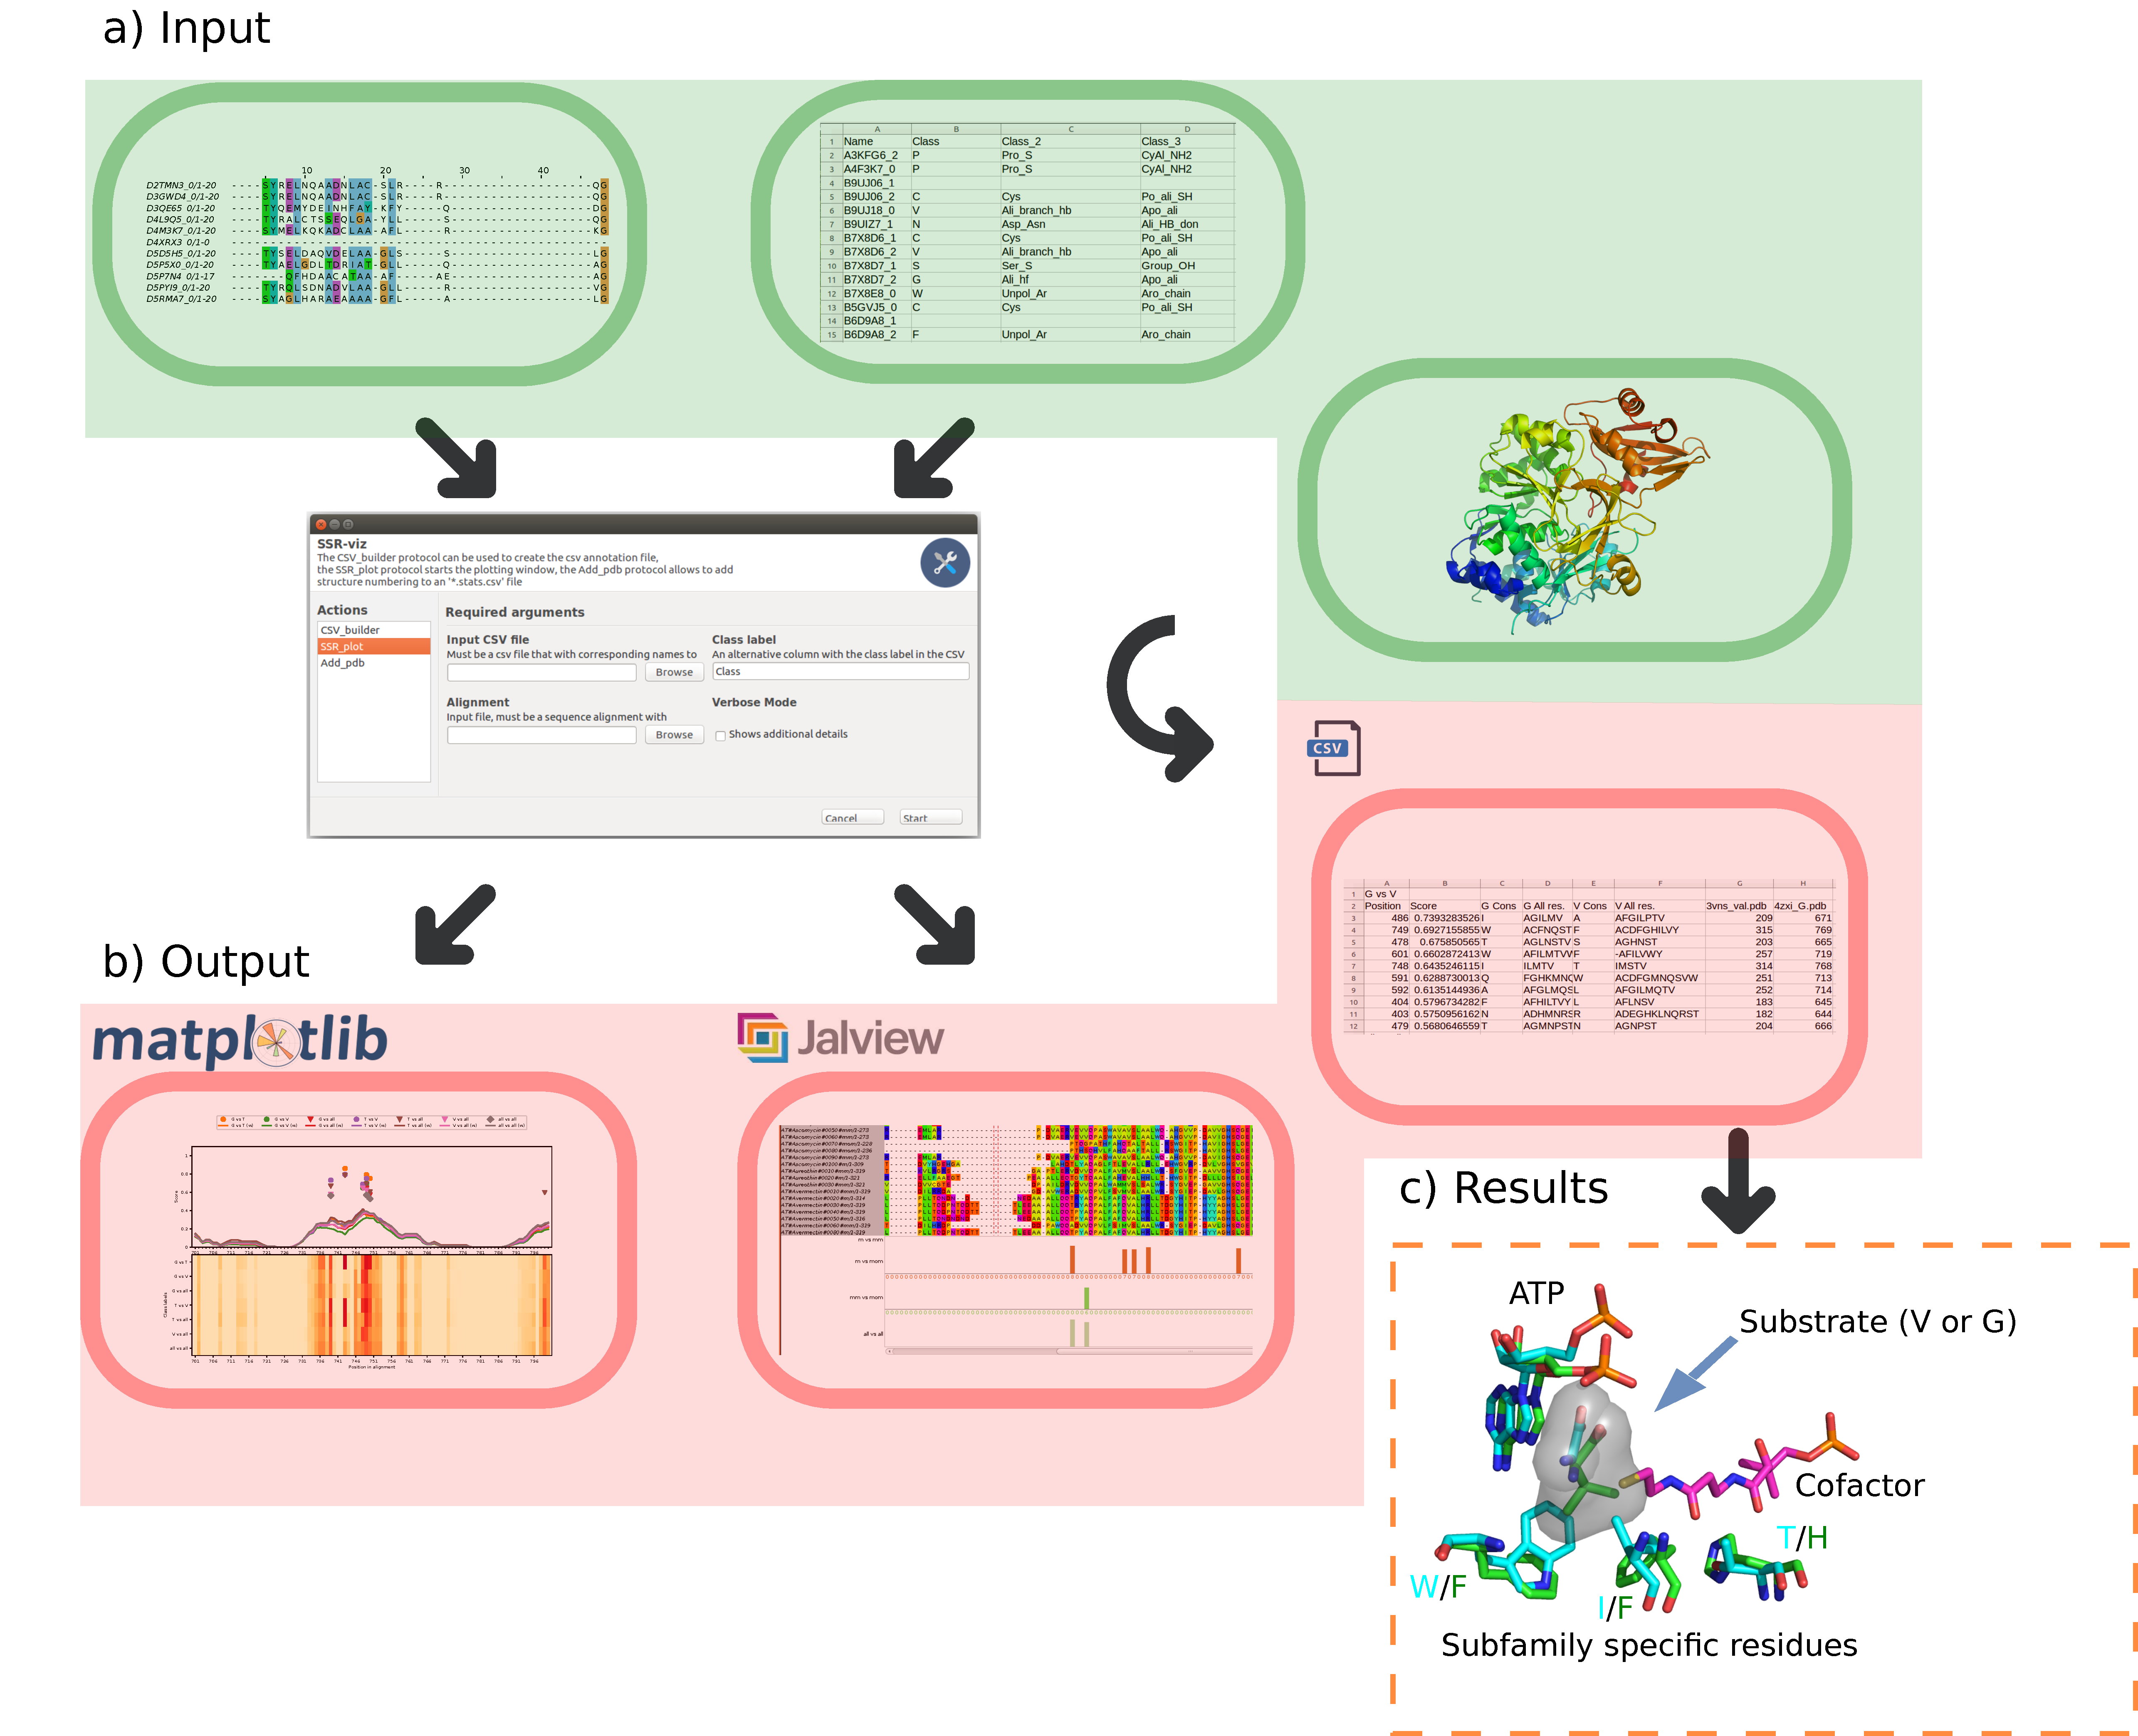
\includegraphics[width=\linewidth]{./figs/flow_chart}
  \caption{General flow chart of the SSR-viz toolbox. a) The input consists 
of a MSA together with a CSV-file holding the corresponding subfamily class labels. 
Multiple protein structures can also be included in order to assign the 
structure indices. b) The output can be created as a mathplotlib PDF, a Jalview annotation file
or a summary CSV-File. This file is used to assign the indices of the structure.
c) Example assignment of SSRs for the NRPS adenylation domain with specificity for Valine and Glycine.}
  \label{fig:flow_chart}
\end{figure}

\section{Algorithm} \label{algo}

The alignment is split into groups representing each protein subfamily as defined in the 
subfamily class label CSV file.
For each group a position probability matrix (ppm) is generated (see eq.\ref{eq:ppm}).
This represents the alignment in form of the probability to find each amino acid at a certain position.
In the following equations $\alpha$ and $\beta$ represent PPMs for two different subfamilies. 

\begin{equation} \label{eq:ppm}
PPM(\alpha) =
\begin{blockarray}{cccc}
 & 1 & 2  & m  \\
\begin{block}{c(ccc)}
  A & \alpha_{A1} & \alpha_{A2}  & \alpha_{Am} \\
  R & \alpha_{R1} & \alpha_{R2}  & \alpha_{Rm} \\
  n & \alpha_{n1} & \alpha_{n2}  & \alpha_{nm} \\
\end{block}
\end{blockarray}
\end{equation}

The conservation score (CS) for each group is computed by applying the normalized Shannon entropy
for each subfamily (eq.\ref{eq:sen}). The score is inverted so that 1 means the position highly conserved and 0
the positions is not conserved (eq.\ref{eq:inv}). The mean of both subfamily represents the final CS (eq.\ref{eq:e_comp}).

\begin{equation} \label{eq:sen}
S(\alpha)_m = -\frac{\sum(\alpha_n*\log_2(\alpha_n))}{S_{max}}
\end{equation}

\begin{equation} \label{eq:inv}
CS(\alpha)_m = 1 - S(\alpha) 
\end{equation}

\begin{equation} \label{eq:e_comp}
CS(\alpha, \beta)_m = \frac{CS(\alpha)_m + CS(\beta)_m}{2}
\end{equation}

The difference of both subfamilies is represented by computing an 
exchange probability matrix of both PPMs (eq.\ref{eq:diff}).
This represents the probability of each residue to be exchanged with another
residues in the other subfamily. The sum of the matrix results in the
exchange probability (EP) score.

\begin{equation}  \label{eq:diff}
EP(\alpha,\beta)_m =
  \sum \sum
  \begin{bmatrix}
    0 & \alpha_{A1} * \beta_{R1} & \alpha_{A1} * \beta_{n1} \\
    \alpha_{R1} * \beta_{A1} & 0 & \alpha_{R1} * \beta_{n1} \\
    \alpha_{n1} * \beta_{A1} & \alpha_{n1} * \beta_{R1} & 0 \\
  \end{bmatrix}
\end{equation}

In order to highlight residues which are exchanged with
residues with different physico-chemical properties, an additionally
score is introduced. Therefore, a weighed exchange matrix (WEM)
is computed based on traditional substitution matrices such as PAM and BLOSUM (eq.\ref{eq:we}). 
The matrix can be chosen as a parameter in the algorithm options.

Based on this matrix the weighed exchange probability (WEP) is computed by multiplying the
EP with the matrix, thereby weighing the exchange differently based on the factor of the WEM (eq.\ref{eq:wep}).
This score is additional weighed with a factor $\gamma$ in order to allow users to define the strength of the 
WEM individually. For some experiments a stronger focus on residues with physico-chemical exchange might be desired.

\begin{equation}  \label{eq:we}
WEM =
\begin{blockarray}{cccc}
 & A & R  & n  \\
\begin{block}{c(ccc)}
  A & 0 & i_{AR}  & i_{An} \\
  R & i_{RA} & 0  &  i_{An} \\
  n & i_{nA} &  i_{nR}  & 0 \\
\end{block}
\end{blockarray}
\end{equation}

\begin{equation} \label{eq:wep}
WEP(\alpha,\beta)_m = \sum\sum (EP(\alpha,\beta)_m * WEM) * \gamma
\end{equation}

The final subfamily specific residue (SSR) score of position m ($ES_m$) is computed by 
summation of all three individual scores.
\begin{equation}
SSR_{score}(\alpha, \beta)_m = CS(\alpha, \beta)_m * EP(\alpha, \beta)_m * WEP(\alpha, \beta)_m 
\end{equation}

An example for the scoring algorithm can be seen in figure~\ref{fig:scoring_02bigger}.

\begin{figure}
  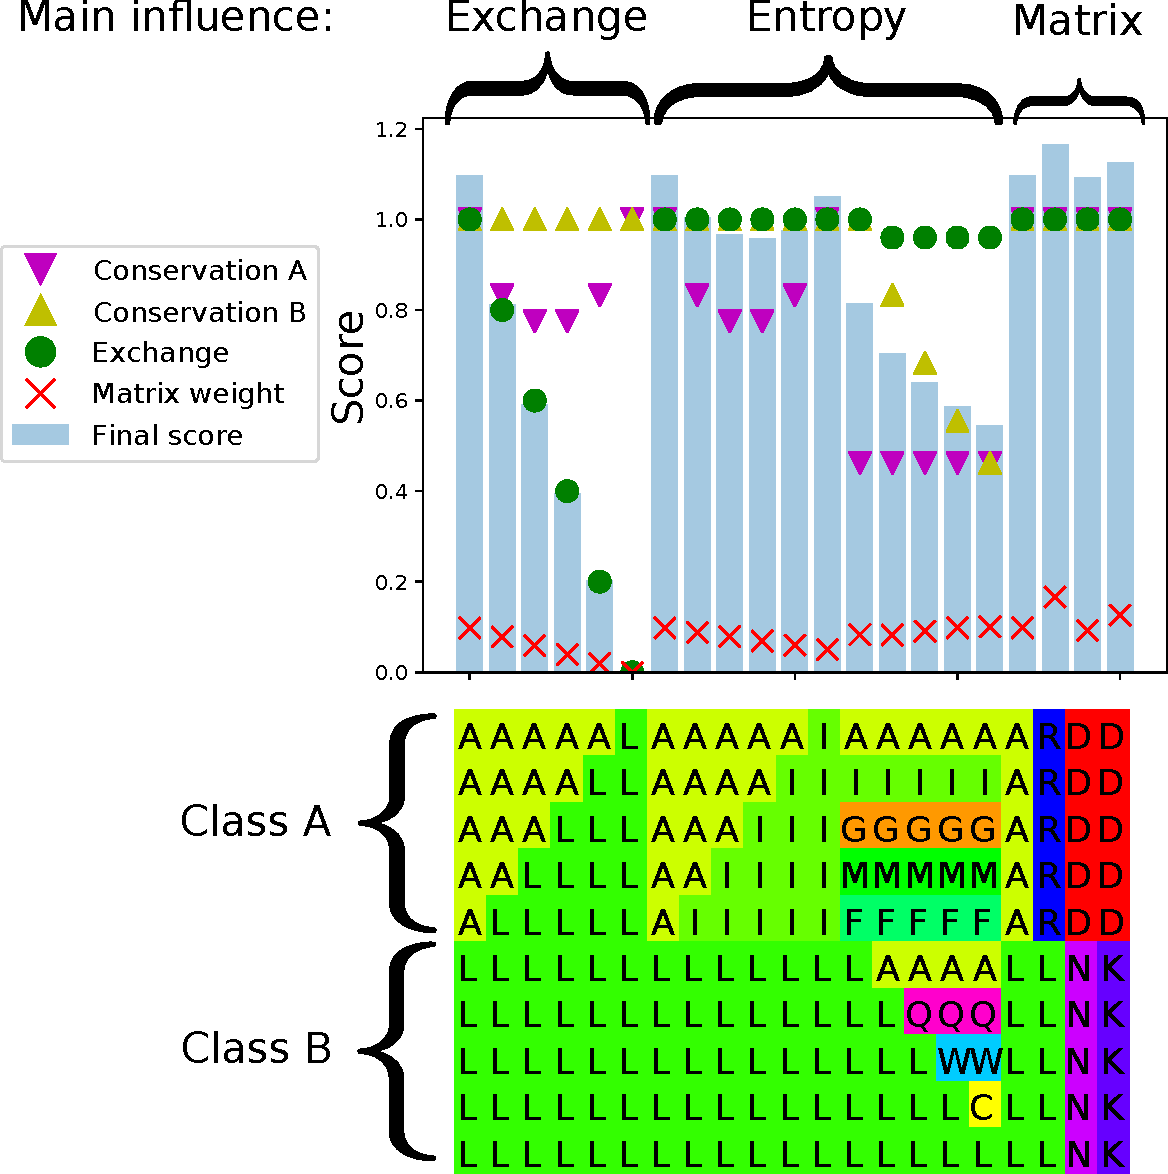
\includegraphics[width=\linewidth]{./figs/scoring_02bigger}
  \caption{
  
  }
  \label{fig:scoring_02bigger}
\end{figure}

\section{CSV builder} \label{csv_b}

The \textbf{CSV\_Builder} handles the input and takes care, 
that the alignment and CSV class label file have the right formating.

\subsection{Arguments}

\begin{description}

\item[\texttt{Input sequence alignment file}] \hfill \\
 
The alignment file with the sequences of the family.
The desired format is in FASTA format (clustalo), see section~\ref{example}
for an example.

\item[\texttt{Inplace FASTA conversion / Temporary alignment file name}] \hfill \\
 
The \textbf{CSV\_Builder} routine will remove duplicates from the 
alignment, as multiple identical sequences will overestimate the importance
of this subfamily. The alignment can be converted inplace, meaning
the original alignment is overwritten or a new alignment can be 
created.

\item[\texttt{Regex extraction of the class label}] \hfill \\
 
The normal \textbf{CSV\_Builder} routine will create a CSV file,
with an empty column for the class labels. Which must be manually 
filled.
In some cases the class labels are part of the sequence names,
this labels can be extracted using regular expressions (regex) patterns.
The entire scope of regex is to big for this manual, but the set of
examples in the appendix~\ref{appendix} should help to get started. There are various 
tools available which can be used to test regex before usage, most text editors 
support regex as a search option. You can 
for example load the alignment file into sublime or notepad, then
search with regex and if the pattern is correct, it should only highlight 
the desired class label. An example is shown in appendix~\ref{appendix}.

\item[\texttt{Output}] \hfill \\

The name of the CSV file, by default it will be created in the same folder as
the sequence file.

\item[\texttt{Delete}] \hfill \\

Allows to overwrite existing CSV files.

\end{description}

\section{SSR plot} \label{ssr_p}

As soon as the alignment file and the class label csv file are created, the detection of
significant SSRs can be performed. 
Therefore, the alignment and the CSV file need to be loaded with the SSR\_plot panel,
if they are loaded correctly, an additional window will open, which allows to set the parameters 
for the detection algorithm and the output options.

\subsection{Arguments}

\begin{description}

\item[\texttt{Input CSV file}] \hfill \\
 
The CSV file holding the class labels. 

\item[\texttt{Class label}] \hfill \\
 
The name of the column holding the subfamily class label information, normally this should just be called "Class",
but an alternative column name can also be chosen, in order to use alternative class definitions. See also:
\ref{example}.

\item[\texttt{Alignment}] \hfill \\

The alignment file used to create the CSV file. Different alignments can be chosen in oder to 
observe influence of the alignment parameters or the alignment algorithm. But the names of the sequences in 
the file need to match the names in the CSV file.

\item[\texttt{Verbose}] \hfill \\

Shows some additional informations about the loading process, for example which files do not match between CSV and alignment file.
(Ideally this should not happen.)

\end{description}

\section{SSR draw} \label{ssr_p}

In this new window all parameters for the algorithm and the output can be adjusted. Each time the start button is pressed
the SSRs are computed based on the current parameters.

Most of the arguments are self-explanatory, therefore only the more advanced options will be explained in the following
argument list.

\subsection{Arguments}

\subsubsection{File}

\begin{description}

\item[\texttt{File name}] \hfill \\

In many cases it is useful to compute multiple plots and files in order to compare the output with each other.
The computed files have the "file name" argument as prefix. Various runs can be performed
successively by tuning the parameters and changing the file name for each run.
 
\end{description}

\subsubsection{Algorithm}

Here the basic parameters for the algorithm can be set, see also \ref{algo}.

\begin{description}

\item[\texttt{Outliers threshold}] \hfill \\

In order to detect the most significant positions a detection threshold can be set, based on the Z-score,
see \url{https://en.wikipedia.org/wiki/Standard_score}. 
 
\item[\texttt{Best positions}] \hfill \\

A more simple, but less significant approach to filter the most important SSRs can be done by simply setting a 
threshold for the best positions, this approach will always return a set of residues. 

The Z-score and Best positions argument can also be set together.

\item[\texttt{Gap importance}] \hfill \\

The implemented algorithm considers gaps as a kind of special amino acid, they are assigned a positions in the replacements matrices.
It is difficult to judge the importance of gaps for the detection of SSRs. For example, if a conserved position in protein class A, is 
exchanged with a gap in protein class B, this could be an important information or it could be due to the alignment algorithm.
Therefore, we decided to let the user judge the gaps individually. If the "gap importance" is set to 0, an exchange with an gap will be considered as
unimportant. If the "gap importance" is set to 1 it is considered as an most important amino acid exchange. The influence of the gap can be judged
by running the algorithm with both settings each and comparing, if the significant positions are changed.

\item[\texttt{Matrix}] \hfill \\

This allows to choose the substitution matrix used for the algorithm (see \ref{algo}), all matrices which are implemented in Biopython can be used,
see \url{http://biopython.org/DIST/docs/api/Bio.SubsMat.MatrixInfo-module.html} for details. 

Additionally, we computed a substitution matrix purely based on the physico-chemical properties of the amino acids, based on (\todo{cite}). 

\item[\texttt{Weight of the replacement matrix}] \hfill \\

The basic algorithm computes the most significant residues to distinguish protein subfamilies. 
Amino acid properties are not considered for this analysis. In many cases
even residues which are very similar can have a great influence on protein function, in other cases
the have no influence at all. Therefore, we allow the user to decide how important the substitution matrix should be
weighed. 
The default parameter of 0.01 is usually a good start. This will only little influence the initial order of the residues,
but for those residues with the same score, they will be reordered with a higher focus on residues replaced with more different residues.
See also \ref{algo} and \ref{example}.

\end{description}

\subsubsection{Figure}

Here the created visualization can be adjusted, in order to create nice looking plots.
The output figure consists of two parts, a heatmap of the SSRs and a plot 
with the most significant positions on top (see figure \ref{fig:plot_example}).
 
\begin{figure}
  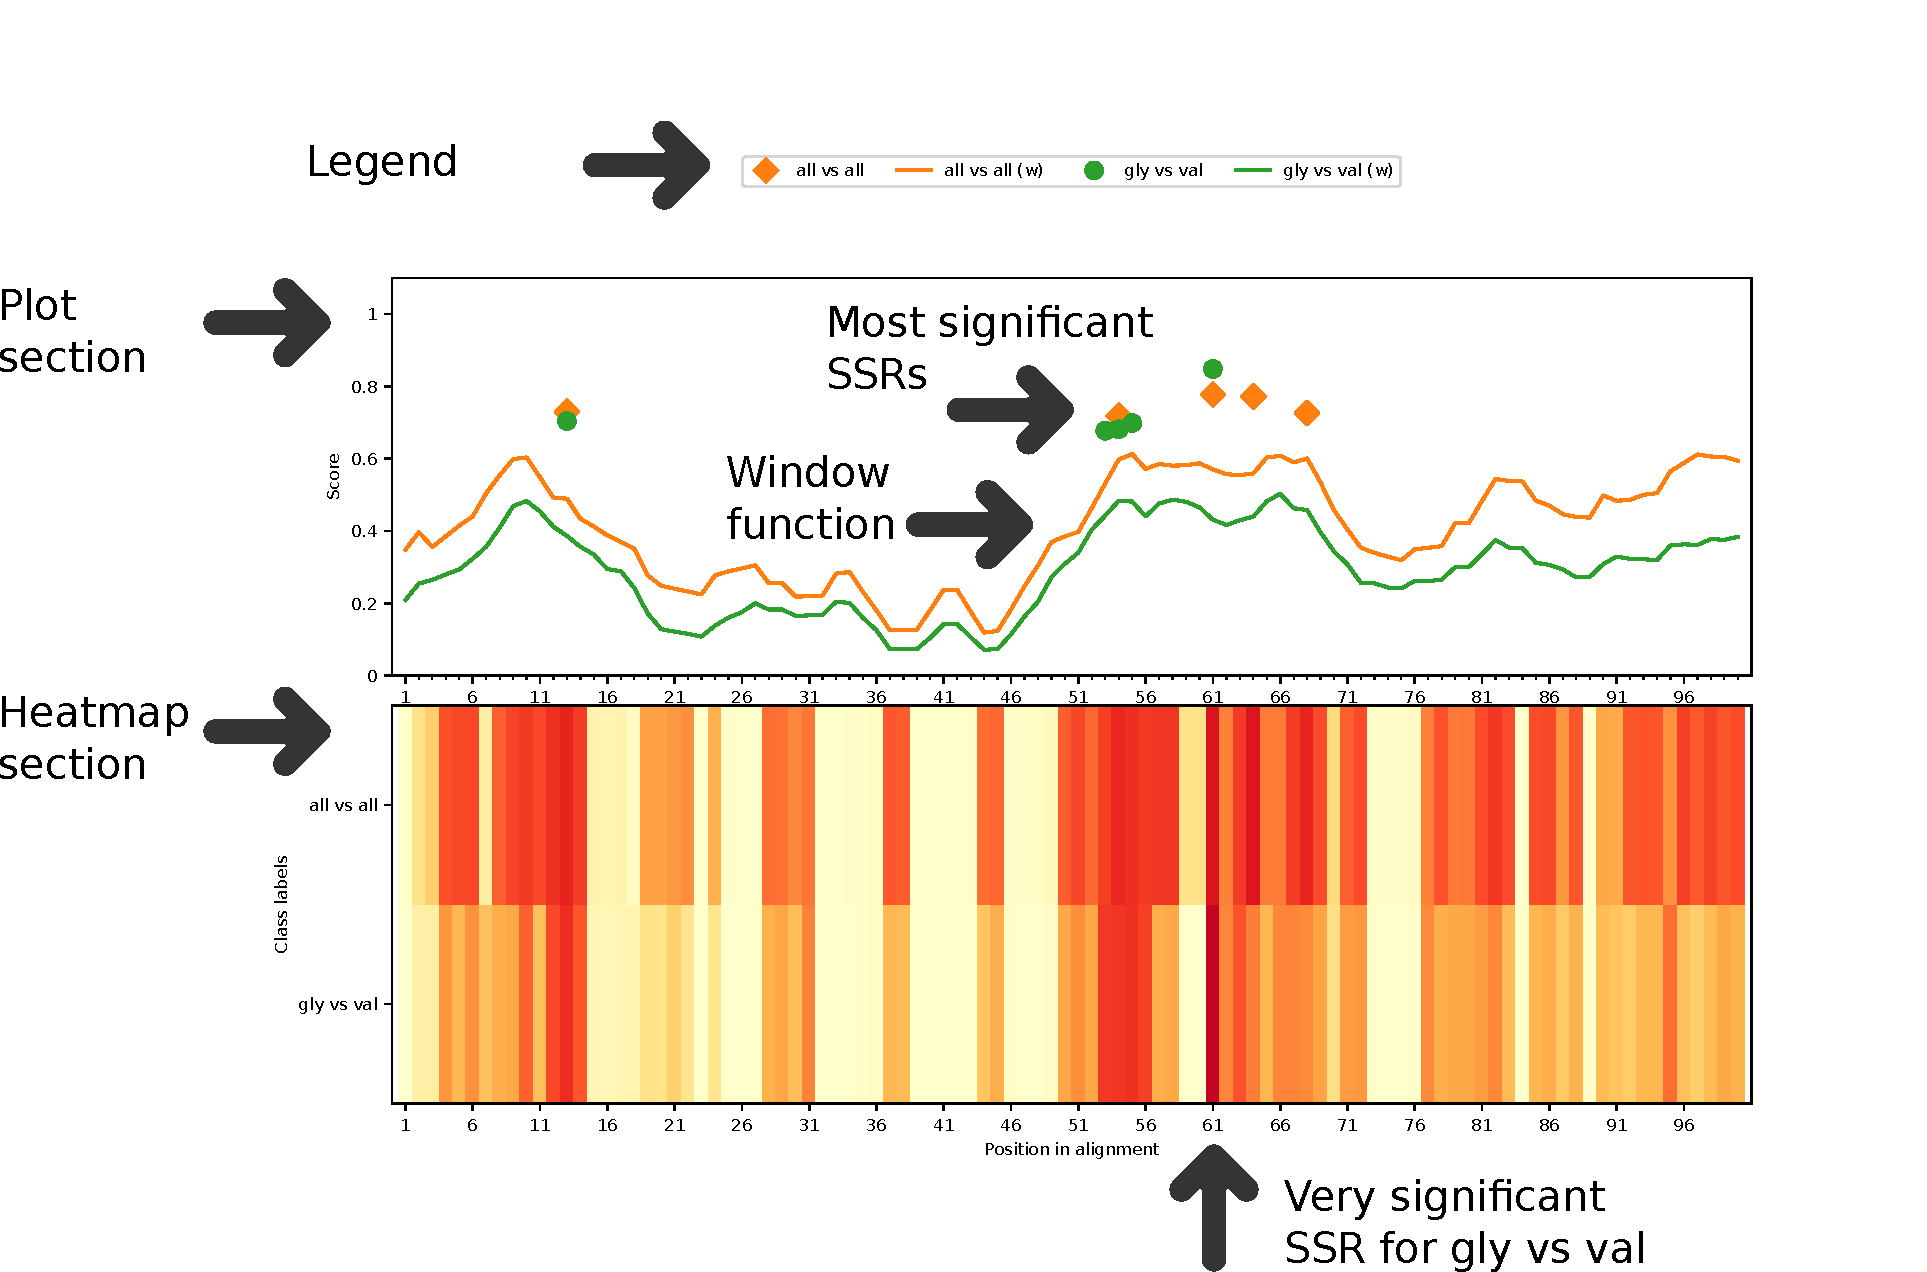
\includegraphics[width=\linewidth]{./figs/plot_example}
  \caption{Example SSR-viz output: The SSRs are computed for the adenylation domain of the NRPS system. 
  The subfamily classes are defined according to the substrate specificity of the domain: glycin (gly) and valine (val).
  See also the example in Section~\ref{example}.}
  \label{fig:plot_example}
\end{figure}

Keep in mind that for projects with multiple protein sub-families the plots can be 
easily overcrowded. A maximum of 10 panels for the heatmap and 5 panels for the plot are 
recommended.

\begin{description}

\item[\texttt{Remove label from top of plot}] \hfill \\

Usually a legend is plotted on top 
\todo{should be legend instead of label} of the plots, this looks only nice for about 5 or 6 labels.
It can be removed, but the recommended way is to plot the SSRs for less subfamilies. 

\item[\texttt{Figsize hight / Figsize width}] \hfill \\

The default figure size is Din A4 but any other size can be chosen.

\item[\texttt{Chunk size of the figure}] \hfill \\
 
How many residues should be plotted per page. 

\item[\texttt{Entire alignment in one plot}] \hfill \\

This argument would squeeze the entire alignment in one plot, 
which can be useful to get on overview of the alignment.

\item[\texttt{Tick positions}] \hfill \\

How often the positions should be shown in the bottom ticks.

\item[\texttt{Ratio plot / ratio heatmap}] \hfill \\

Sets the ration between plot and heatmap.

\end{description}

\subsubsection{Additional output}

Additionally to the created figure, two additional outputs can be created:

\begin{description}

\item[\texttt{Jalview annotation file}] \hfill \\

This file can be imported to Jalview, so that the SSR scores can 
be visualized together with the alignment. Just open the alignment with Jalview and 
click File, then Load Features/Annotations and then choose the created *.jv\_plot.txt 

\item[\texttt{Plot statistics}] \hfill \\

This creates a csv file, which shows tabular informations of the SSRs created. 
The file lists the significant positions for each scoring scheme, including the positions in the alignment,
the score, the conserved residue and the entire variety of residues for each subfamily. 

\end{description}

\subsubsection{Plot Options}

Here the plot output can be modified.

\begin{description}

\item[\texttt{Window size / Window type}] \hfill \\

Additionally to the most significant positions, the plot can also apply a window function to the SSRs.
This window function can be used to visualize general ares of interest in the alignment. 
Possible windows are: mean, max, min, std. 
If the window is set to 1 it shows you the exact SSRs for each residue.

\item[\texttt{No all vs all plot}] \hfill \\

Besides the chosen one-vs-one and one-vs-all schemes, the plot always shows the SSRs for the all-vs-all scheme, representing the residues
which are most important to distinguish all subfamilies from each other. This can be removed with this option.

\end{description}

\subsubsection{One-vs-One plot}

Here are all the subfamilies listed which were parsed from the subfamily class label CSV-file. 
Each can be choses to compute the SSRs. Keep in mind, that an all-vs-all scheme can become very large, as each
subfamily will be compared to each other. Best practice would be to concentrate on a few (3-4) subfamilies and create multiple plot.

\subsubsection{One-vs-All plot}

The choice is identical to the One-vs-one plot, but shows the SSRs most significant to distinguish each subfamily from all the other 
subfamilies.

\subsubsection{Heatmap Options}

\begin{description}

\item[\texttt{No all vs all row in the heatmap}] \hfill \\

Besides the chosen one-vs-one and one-vs-all schemes, the heatmap always shows the SSRs for the all-vs-all scheme, representing the residues
which are most important to distinguish all subfamilies from each other. This can be removed with this option.

\item[\texttt{Remove the labels from the heatmap}] \hfill \\

The labels can be removed from the heatmap. For example if very much one-vs-one schemes are shown, it looks better without labels.

\end{description}

\subsubsection{One-vs-One Heatmap}

Identical to One-vs-One plot, but for the heatmap.

\subsubsection{One-vs-all Heatmap}

Identical to One-vs-All plot, but for the heatmap.

\section{Add pdb} \label{add_p}

\subsection{Arguments}

\section{Example} \label{example}

\section{Appendix} \label{appendix}

\subsection{Regex examples}

% Example 1
% 
% > sequence1\_spec_ATP
% > sequence2\_spec_ADP
% > sequence3\_spec_ADP
% > sequence4\_spec_ATP
% > sequence5\_spec_ATP
% 
% Possible Regex: ''\_([ATDP]+)\$'' 
% 
% Example 2
% 
% > sequence1\#1
% > sequence2\#3
% > sequence3\#1
% > sequence4\#3
% > sequence5\#4
% 
% Possible Regex: ''\#([1-9])\$'' 
% 
% Example 1
% 
% > class:mm_sequence1
% > class:mom_sequence2
% > class:mm_sequence3
% > class:mm_sequence4
% > class:mal_sequence5
% 
% Possible Regex: ''class:([a-z]*)_'' 


\end{document}
